\documentclass[../../main.tex]{subfiles}

%-----------------------------------------------------------%
\begin{document}
\subsection{Tracking Mode}

\subsubsection{Introduction}
Tracking Mode is the primary operating mode of a satellite (the other being the Lost-in-Space Mode, which is generally a rare event in the lifetime of a standard operating star tracker), wherein the attitude of the satellite is already known. The main objective of tracking mode is to perform Star Matching using the \textit{a priori} attitude information to decrease the computation time as compared to the Lost-in-Space Mode for successfully matching observed stars with their true Star-IDs (from the pre-loaded Star Catalogue). 

\subsubsection{Literature Survey}
After an extensive literature survey on Tracking Mode algorithms, a few algorithms were shortlisted based on the number of citations, space heritage, ease of implementation and the year of publication. Some papers were survey based papers which documented an extensive study on different algorithms proposed till date. Many algorithms were shortlisted based on the results shown in these papers. These algorithms are mentioned in detail below. 

\subsubsection{Recursive Mode Star Identification Algorithms}
% hey, don't write "This Paper", instead write "This algorithm \cite{ref} proposes ...."
This paper proposes two methods for recursive mode star identification, the Spherical Polygon search (SP-search) and the Star Neighbourhood Approach (SNA). Once the Lost In Space Algorithm (LISA) has been executed for a single frame of the star tracker, the proposed algorithm (SNA or SP Search) is used to obtain expected stars in the FOV from the Star Catalogue for the next frame. These expected stars form the \textit{Reference Image}.
The Feature Extraction process is executed in the next frame, obtaining the true centroids, which form the \textit{Measured Image}.The Star ID process is completed by matching the inter-star angles between the measured image and the reference image. The two algorithms are explained in detail below. 
\begin{itemize}
    \item \textbf{Spherical Polygon Approach}\\
    \\
    The Spherical Polygon Approach does not require any (accurate or not) initial guess of the spacecraft attitude, and does not use the typically low accuracy magnitude information. The algorithm is recursive in the sense that it matches 3 stars at a time observed in the \textit{Measured Image} till all the observed stars are matched. 
   If \textit{$s_{i}$}, \textit{$s_{j}$}, and \textit{$s_{k}$} are three different observed star directions (unit-vectors), it is always possible to set
   \begin{equation}
        \textit{$s_{k}$} = a\textit{$s_{i}$} + b\textit{$s_{j}$} +c(\textit{$s_{i}$} \times \textit{$s_{j}$})
    \end{equation}
    unless \textit{$s_{i}$} and \textit{$s_{j}$} are not parallel (i.e. double stars). The a, b and c coefficients represent an invariant set of parameters with respect to the used system of coordinates. This means that there exist, in the Star Catalogue, three stars (\textit{$v_{i}$}, \textit{$v_{j}$} and \textit{$v_{k}$}) such that condition (10.1) holds as,  
    \begin{equation}                    
        \textit{$v_{k}$} = a'\textit{$v_{i}$} + b'\textit{$v_{j}$} +c'(\textit{$v_{i}$} \times \textit{$v_{j}$})
    \end{equation}
    where the a', b', and c' coefficients will differ from the a, b, and c coefficients because of the sensor’s limited precision, that is, because the observed stars directions do not perfectly overlap with the catalog star directions.\\
    The algorithm uses the \textbf{\textit{k}-vector} range searching technique twice to finally match a triad of observed stars. Based on these facts, the algorithm follows the following steps:
    \begin{enumerate}                   
        \item The first instance of the use of \textbf{\textit{k}-vector} is to find all the catalogue star pairs (\textit{$v_{i}$} and \textit{$v_{j}$}) admissible with the observed star pair \textit{$s_{i}$} and \textit{$s_{j}$}.
        \item For each possible pair of catalogue stars, there exists a corresponding solution for the true catalogue star \textit{$v_{k}$} associated with the observed \textit{$s_{k}$} star.
        \item To find the true solution for \textit{$v_{k}$} out of all possible solutions, it has to be searched within a cone of aperture h$\sigma$ around each solution, which is done using the \textbf{\textit{k}-vector} technique.
        \item This is accomplished by approximating the observed cone area as the area covered by a spherical polygon, which is identified as the intersection of six cones, as shown in fig. 10.6
        \item The SPS procedure has a successful end if only one star falls within one of the cones of aperture h$\sigma$. When this occurs, the triad (\textit{$s_{i}$}, \textit{$s_{j}$}, \textit{$s_{k}$}) is matched with the triad (\textit{$v_{i}$}, \textit{$v_{j}$}, \textit{$v_{k}$}). 
    \end{enumerate}
    \begin{figure}[!h]
        \centering
        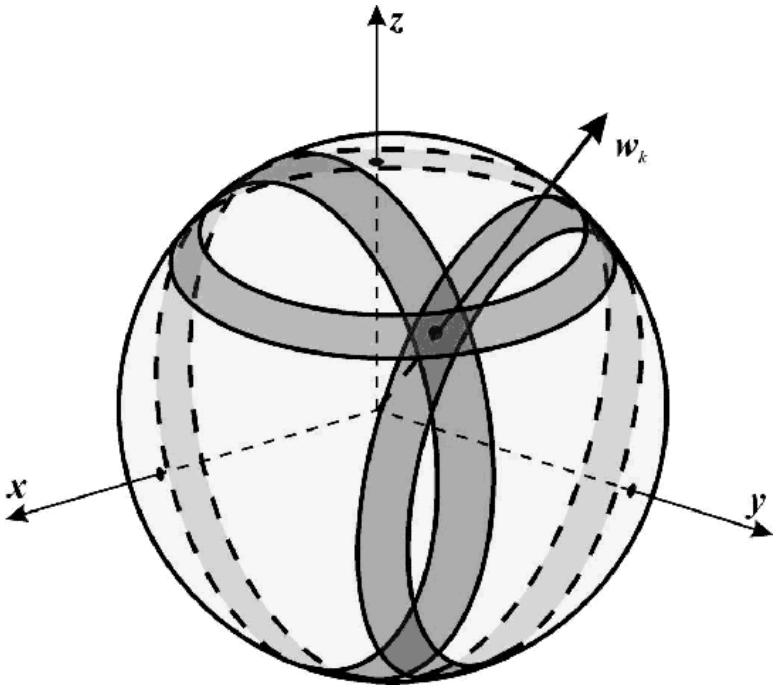
\includegraphics[scale=0.35]{Figures/GNC/sp_search.png}
        \caption{Spherical Polygon}
        \label{fig:sp_search}
    \end{figure}
    
    \item \textbf{Star Neighbourhood Approach} \label{sna}\\
    
    The Star Neighbourhood approach is the second recursive algorithm which uses the previously identified stars to access the candidate stars (which form the \textit{Reference Image}) to match with the current observed stars (which form the \textit{Measured Image}). This approach makes use of the spacecraft attitude at each frame (obtained by estimating the Angular Velocity from the Gyroscope) and the previously identified Star IDs. The steps of the algorithm are detailed below:
    \begin{enumerate}
        \item The LISA is run for the first time which determines the \textbf{attitude matrix} and \textbf{Star-IDs} at time $t_{0}$.
        \item \textbf{Simulation of Stars}
        By knowing the attitude matrix at each time step we can calculate the normal vectors to the sensor frame in the body frame, which is known as the 'Bore-sight vector', to simulate the frames of stars at the next time step, i.e, create a simulation of the actual image which will contain catalogue stars and place them at positions at which the 'true centroids' should ideally be found (\textit{Reference Image}).
        \item \textbf{Star Mapping}
        The simulated star unit vectors are converted to image plane coordinates ($x_{i}$, $y_{i}$)using the following formula:
        \begin{equation}
            x_{i} = -f\frac{x^{T}b_{i}}{z^{T}b_{i}} \hspace{3em} y_{i} = -f\frac{y^{T}b_{i}}{z^{T}b_{i}}
        \end{equation}
        where \textbf{$C^{T}$ = [x,y,z]} is the sensor attitude matrix, \textbf{$b_{i}$ (i=1,2,3.....n)} are the simulated star vectors and \textbf{f} is the camera focal length. 
        \item \textbf{Star Spot Prediction}
        The estimated location of star i at the current frame ($x_{i}$, $y_{i}$)$_{t+\delta t}$ is calculated by adding the location of star i at the previous frame ($x_{i}$, $y_{i}$)$_{t}$ and estimated translation of the frame $\omega\delta$t.
        \item \textbf{Star Matching} Now the estimated locations of stars (Reference Image) is matched with the measured locations of stars (Measured Image) using a Radius based approach as shown in figure (10.7). 
        \begin{figure}[!h]
        \centering
        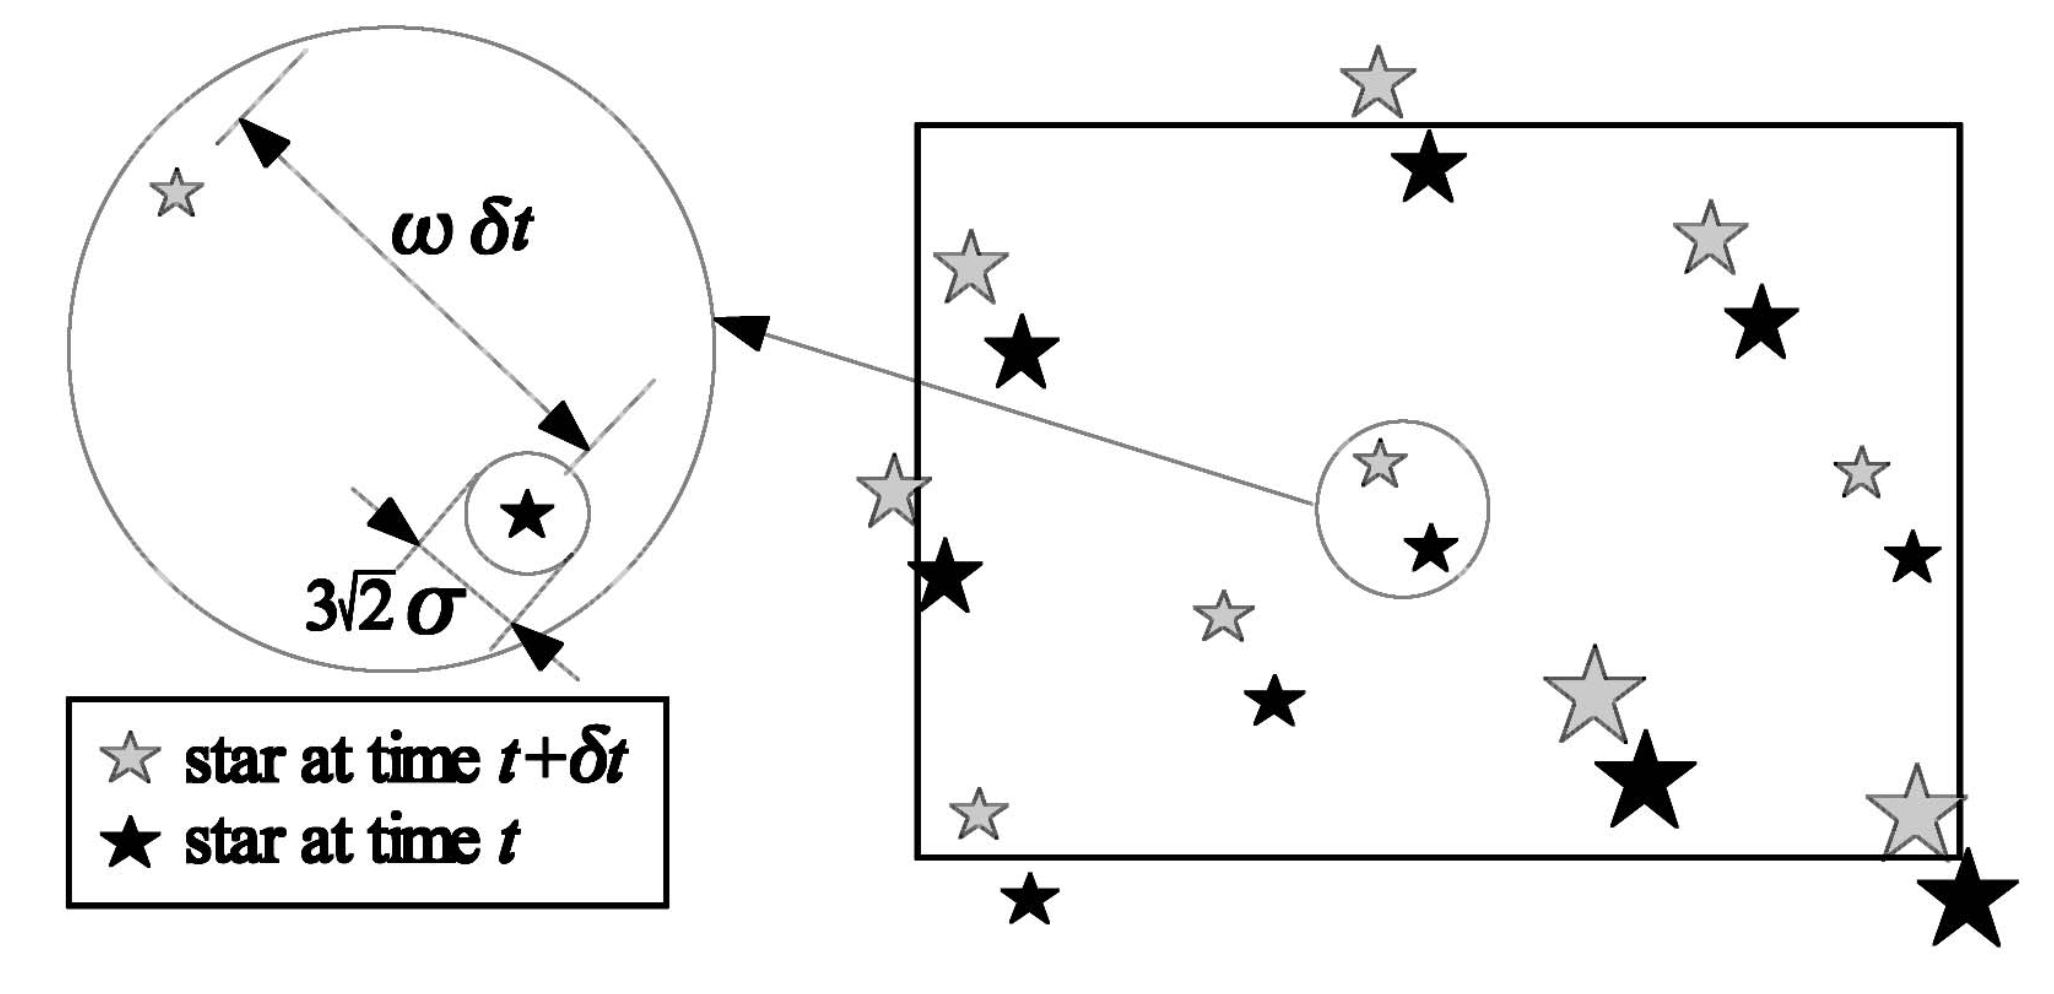
\includegraphics[scale=0.20]{Figures/GNC/radius_matching.png}
        \caption{Radius Based Matching}
        \label{fig:radius_based_sna}
        \end{figure}
        \item For the unmatched stars from steps 4 and 5, the \textbf{Star Neighbourhood Table} is used to identify the stars which enter the sensor frame at ($t+\delta t$), by checking the inter-star angles between the unmatched stars and their matched star neighbours. 
    \end{enumerate}
    The logic for the SNA is shown below:
    \begin{figure}[!h]
        \centering
        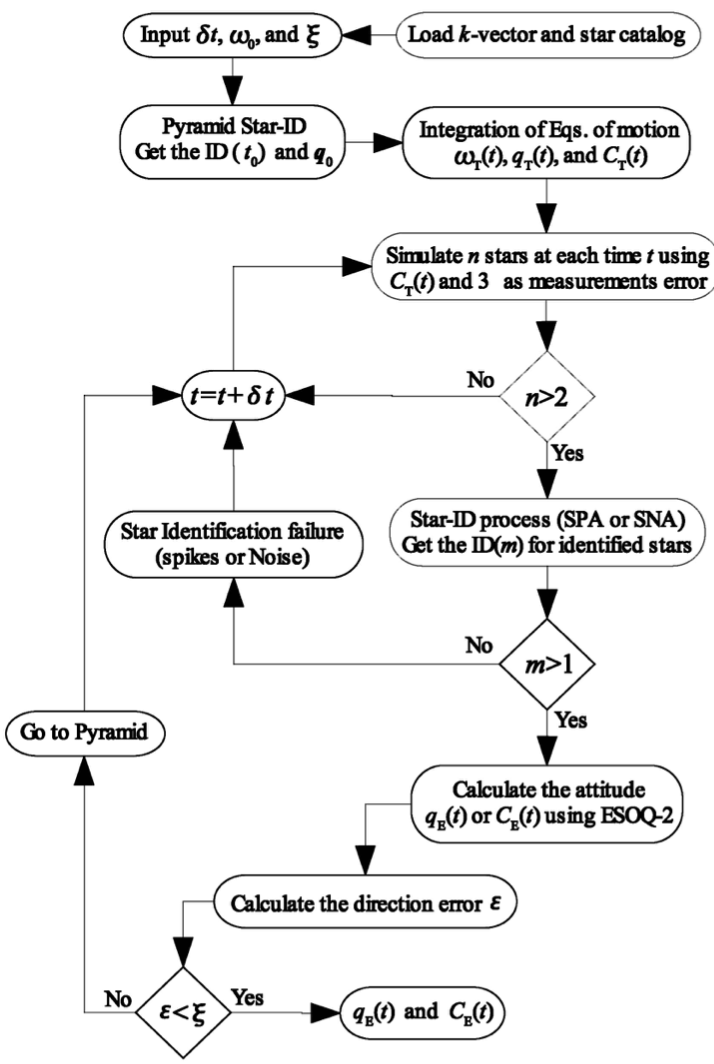
\includegraphics[scale=0.5]{Figures/GNC/sna_flowchart.png}
        \caption{Logic Flow Diagram - SNA algorithm}
        \label{fig:sna_flowchart}
    \end{figure}
\end{itemize}

\subsubsection{Rapid Star Tracking Algorithm} \label{rapidtrack}
This algorithm does not require any previous attitude information or an estimate of the angular velocity of the spacecraft, unlike the previous algorithm. Instead, it only uses the previously identified stars' information (Right Ascension, Declination, Star ID) to track stars in the current frame. Before understanding the details of the algorithm, some terms are introduced:
\begin{itemize}
    \item \textbf{Reference Image} : The image from the previous frame where all the observed stars have been identified.
    \item \textbf{Observed/Measured Image} : The image at the current frame where only the centroid information is known, and the task at hand is to correctly identify these centroids using the information of the Reference Stars (in the Reference Image). 
\end{itemize}
The principle of the algorithm is detailed step-by-step below:
\begin{enumerate}
    \item The star images at the $(k-1)^{th}$ frames and before have been identified, and the objective is to identify the Observed Image at $(k)^{th}$ frame. The identified star image at $(k-1)^{th}$ frame is considered as the Reference Image for the $(k)^{th}$ frame. 
    \item The euclidean distance between the stars in the two images is calculated and compared with a \textbf{radius r}, known as the matching radius, to determine if any reference stars fall in the neighbourhood of an observed star, and if yes, how many. 
    \item If a star's neighborhood in the observed image includes only one star in reference image, the star in observation image is matched with the star in reference image and the star in the observation star image is 'tracked' successfully.
    \item If a star's neighborhood in observation star image includes no
    star or more than one star in reference star image, the star is not matched and tracked. 
    \begin{figure}[!h]
        \centering
        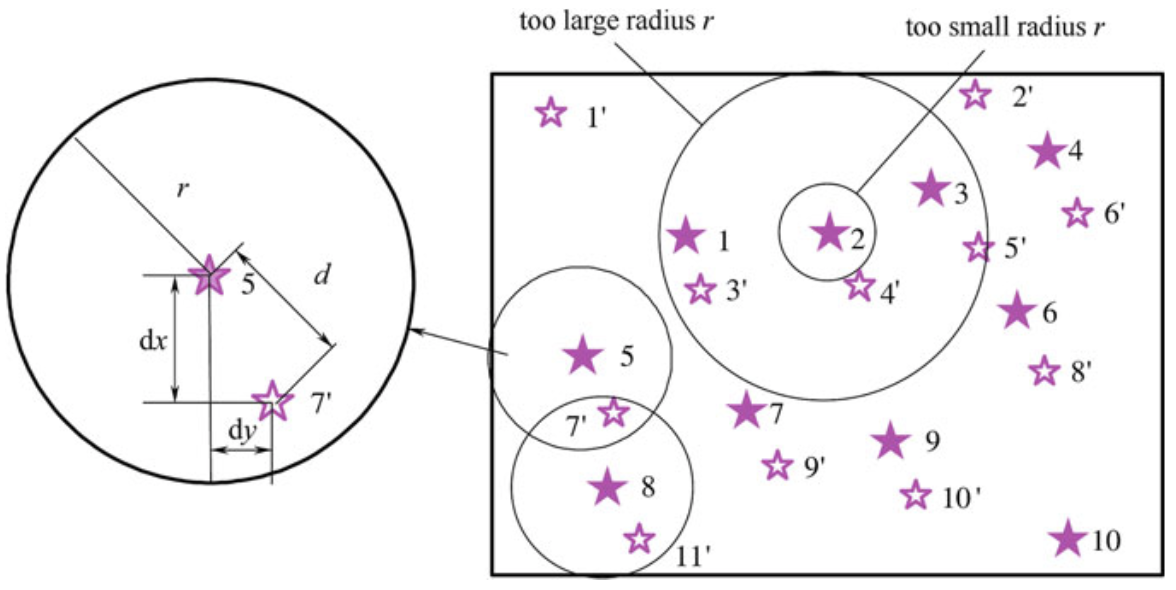
\includegraphics[scale=0.3]{Figures/GNC/radius_based_zhang.png}
        \caption{Radius Based Star Matching}
        \label{fig:radius_zhang}
    \end{figure}
    \item The $(k+1)^{th}$ reference star image can be generated from the tracking results and used to match with the next observation star image in the same way; then stars can be tracked continuously.
    \item Now the stars in the Reference Image will be moved away from the FOV one-by-one. When the stars left in the reference image is less than \textbf{3}, new star identification is necessary, which is done by calculating the star sensor's \textbf{boresight} vector according to the result of the previous tracking, and the stars around the boresight can be obtained from the Star Catalogue.  
    \item The stars vectors obtained from the catalogue in the previous step are obtained from the \textit{Celestial Coordinates} (RA, Dec.) and need to be converted to \textit{Image Plane Coordinates} to start again from step 1. This process is known as \textbf{Star Mapping} is generally a time-consuming task, hence it is executed only when the reference stars are less than 3. 
\end{enumerate}
\begin{figure}[!h]
        \centering
        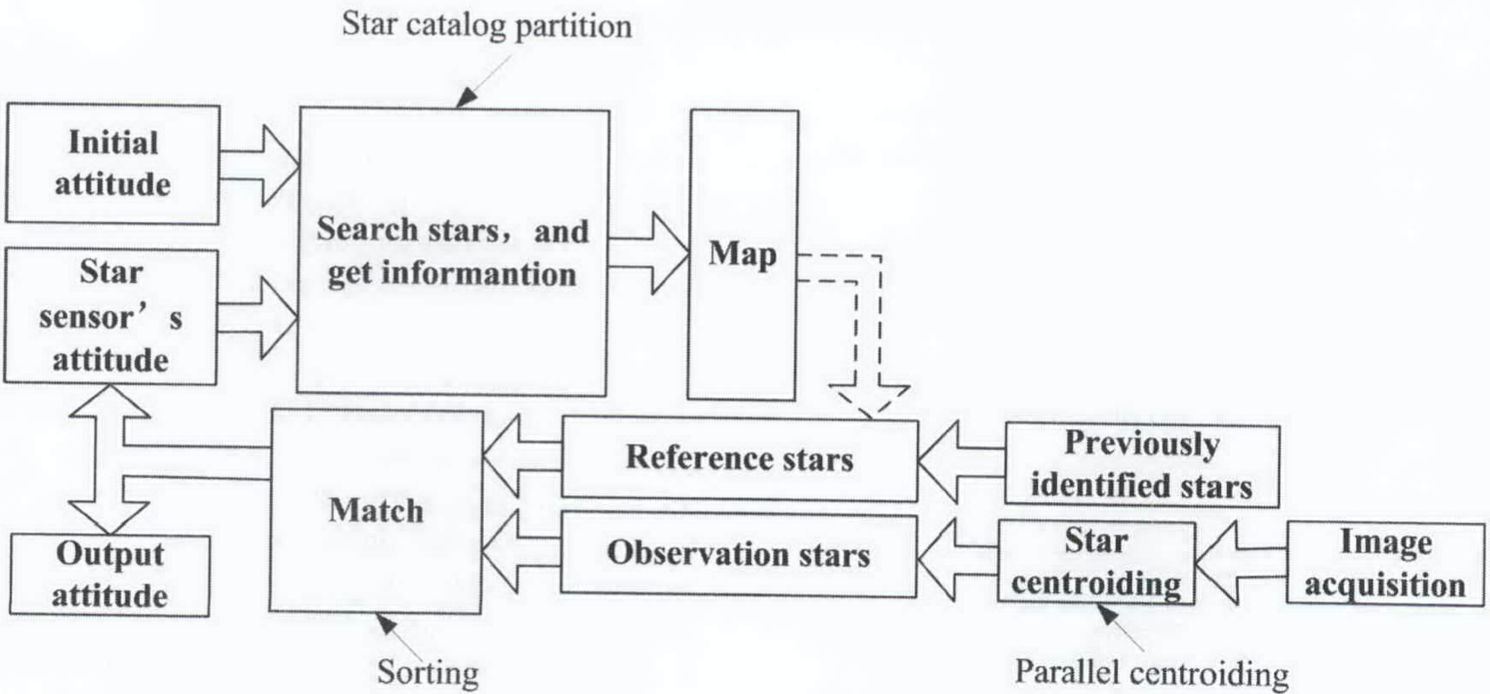
\includegraphics[scale=0.4]{Figures/GNC/rapid_tracking_flowchart.png}
        \caption{Rapid Star Tracking Algorithm Flowchart}
        \label{fig:rapid_tracking_flowchart}
\end{figure}
To speed up the process of star tracking, the algorithm also proposes 3 optimisation techniques. These are explained below:
\begin{itemize}
    \item \textit{Parallel Star Centroiding}:\\
    'Ref pixel by pixel algo from feature extraction'
    
    \item \textit{Sorting Before Matching} \label{sorting_before_matching}:\\
    In step 2 in the algorithm above, the matching between the stars in observation star image and reference star image is implemented one-by-one. But matching between stars with a long distance is meaningless, so sorting before matching is introduced. That is, the stars in the observation image are sorted in ascending order according to their image plane coordinates using bubble sort, and then the matching is carried out. This decreases the number of operations significantly. 
    
    \item \textit{Star Catalogue Partition} \label{catalogue_partition}:\\
    In step 6 and 7 of the algorithm, new star identification is done by accessing catalogue stars using the boresight vector and then mapping them onto the star sensor plane (Star Mapping), which can be time consuming and inefficient if searching for stars through the entire guide star catalogue. This is solved using the concept of \textit{'sub-catalogue'}.
    \begin{itemize}
        \item The celestial sphere is divided into 6 equal zones by using an inscribed cube and then pushing the sides of the cube away from the center of the sphere, to generate 6 equal parts of the celestial spheres. 
        \item Each one of the 6 zones can be partitioned into N x N sub portions. This way, the entire celestial sphere is divided into 6 x N x N sub portions. 
        \item Now all the guide stars can be assigned into these sub portions, instead of their irregular distribution on the whole celestial sphere. This way, if the boresight direction is known in step 6, the sub portion and hence the guide stars around that boresight can be found quickly. The partition table will be pre-processed and stored with the guide catalogue. 
    \end{itemize}
\end{itemize}


\subsubsection{Rapid Star Tracking Using Star Spot Matching Between Adjacent Frames} \label{zhang}
This algorithm is very similar to the 'Rapid Star Tracking Algorithm' with a minor difference being in how the \textbf{Reference Image} is formed at every frame. The algorithm introduces another step, known as \textbf{Star Spot Prediction}, which uses the movement of stars in the previous frames to predict the position of stars in the next frame of star image. The flowchart of the algorithm is shown in Fig. \ref{fig:zhang_tracking_flowchart}.\\
In accordance with the attitude of star sensor, boresight vector of the current frame can be calculated, after which the Star ID process is carried out as described in steps 2, 3 and 4 of section \ref{sna}. 
Star matching between the predicted centroids (Reference Image) and the true centroids (Measured Image) is carried out as shown in Fig. \ref{fig:radius_zhang}. A thing to be noted here is that the 'Matching Radius' used for star matching in this algorithm will be smaller because the reference stars here are the predicted centroids instead of the identified stars of the previous frame. 
\begin{figure}[!h]
        \centering
        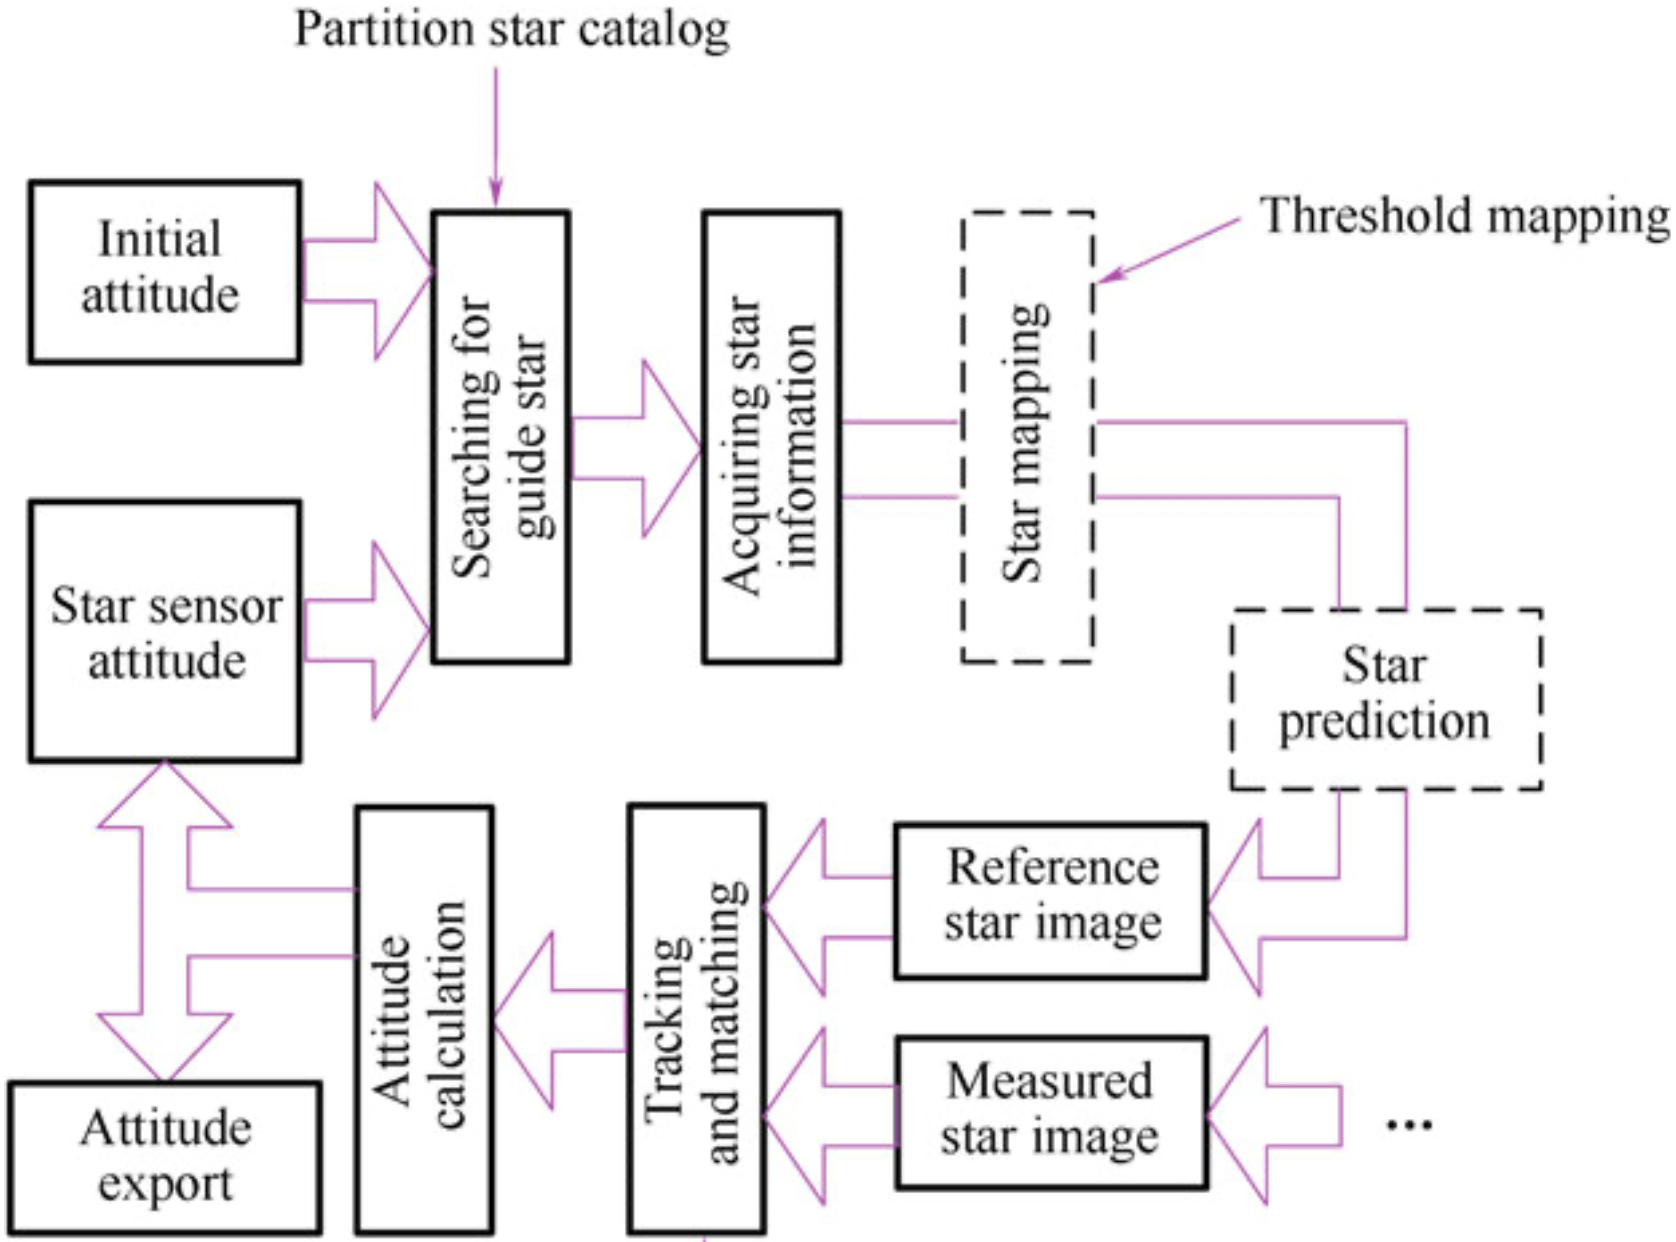
\includegraphics[scale=0.35]{Figures/GNC/zhang_tracking_flowchart.png}
        \caption{Star Tracking Algorithm Flowchart}
        \label{fig:zhang_tracking_flowchart}
\end{figure}\\
This algorithm also proposes three optimisation techniques to speed up the process of star tracking, where \textit{Sorting Before Matching} and \textit{Star Catalogue Partition} are the same as described before in algorithm \ref{rapidtrack}. The third technique, known as \textit{Threshold Mapping}, is explained below: 
\begin{itemize}
    \item \textbf{Threshold Mapping}\\ \label{threshold_mapping}
    In the process of Star Tracking, 'Star Mapping' is the most time consuming process and executing it at every frame defeats the purpose of a tracking mode algorithm. \\
    In Threshold Mapping, a star number threshold, defined as $N_{\textit{TH}}$, is set. Star Mapping is not conducted unless the number of 'Measured' stars tracked successfully is smaller than $N_{\textit{TH}}$. In this event, the measured image at the current frame, with the Star IDs identified, is used as the Reference Image for the next frame, after which Star Matching is carried out again as shown in Fig. \ref{fig:radius_zhang}. Hence, threshold mapping is adopted in order to reduce the frequency of star mapping. The process can be shown in Fig. \ref{fig:threshold_mapping}.
\end{itemize}
% PROBLEM : The figure shows \delta as the threshold whereas we have used Nth in the explanation. 
\begin{figure}[!h]
        \centering
        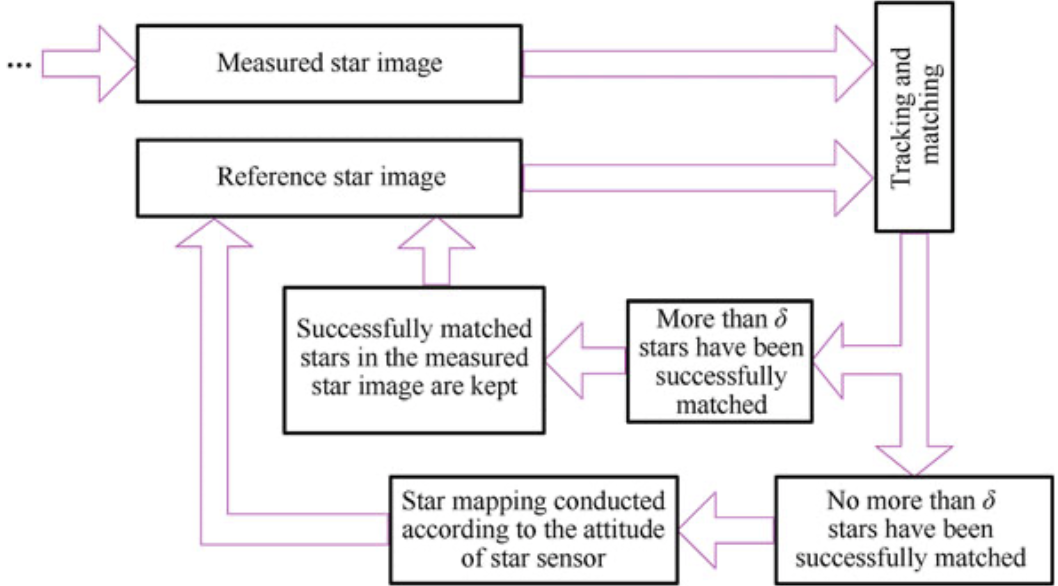
\includegraphics[scale=0.55]{Figures/GNC/threshold_mapping.png}
        \caption{Threshold Mapping}
        \label{fig:threshold_mapping}
\end{figure}


\subsubsection{Fast Star Tracker Centroid Algorithm}
This algorithm proposes a new star tracking algorithm, where the processes of Star Prediction and Star Matching are approached differently as compared to all algorithms discussed before. The algorithm does not require the use of a Gyroscope for obtaining the spacecraft angular velocity or the attitude information of any frame. Instead, the algorithm proposes an 'attitude independent' approach for estimating the angular velocity, i.e, the angular velocity can be estimated even without the attitude information of the current frame, and this estimated angular velocity is then used for centroid prediction. 
\begin{itemize}
    \item \textbf{Angular Velocity Estimation and Centroid Prediction}\\
    The angular velocity estimate is obtained using only the centroid information of the previous \textbf{two} frames. 
    %The process is detailed below:
    % \begin{enumerate}
    %     \item Each star's unit vector can be calculated from its corresponding image plane coordinates by using the following formula:
    %     \begin{equation}
    %         \begin{bmatrix}
    %         x\\y\\z
    %         \end{bmatrix} = \frac{1}{\sqrt{u^2 + v^2 + f^2}} 
    %         \begin{bmatrix}
    %         u\\v\\f
    %         \end{bmatrix}
    %     \end{equation}
    %     where f is the lens focal length, and (u,v) are the image plane coordinates.
    %     \item Now, recalling Euler's Rotation Matrix (or Direction Cosine Matrix or DCM) from one reference frame to another: 
    %   \footnotesize{ \begin{equation}
    %         DCM = 
    %         \begin{bmatrix}
    %         cos(\psi)cos(\theta) & sin(\psi)cos(\theta) & -sin(\theta) \\
    %         -sin(\psi)cos(\phi)+ cos(\psi)sin(\theta)sin(\phi) & cos(\psi)cos(\phi)+sin(\theta)sin(\psi)sin(\phi) & cos(\theta)sin(\phi)\\
    %         sin(\phi)sin(\psi)+cos(\psi)sin(\theta)cos(\phi) & -cos(\psi)sin(\phi)+sin(\phi)sin(\theta)cos(\phi) & cos(\theta)cos(\phi)
    %         \end{bmatrix}
    %     \end{equation}
    %     }\\
    %     \normalsize 
    %     \begin{equation} \label{dcm_rotate}
    %         \begin{bmatrix}
    %         x\\y\\z
    %         \end{bmatrix} = DCM 
    %         \begin{bmatrix}
    %         x_{o}\\y_{o}\\z_{o}
    %         \end{bmatrix}
    %     \end{equation}
    %     where \textbf{$\phi$} is roll in radians about the x-axis, \textbf{$\theta$} is pitch in radians about the y-axis, and \textbf{$\psi$} is yaw in radians about the z-axis.  
        
    %     \item Assuming the small angle approximation, ($sin(\omega) = \omega$, $cos(\omega) = 1$ ; $\omega\psi = 0$; $\omega$ and $\psi$ $<<$ 1), \\
    %     Euler's equation can be reduced:
    %     \begin{equation}
    %         DCM \approx
    %         \begin{bmatrix}
    %         1 & \psi & -\theta \\ -\psi + \theta\phi & 1 + \theta\psi\phi & \phi \\
    %         \psi\phi+\theta & -\phi + \theta\psi & 1 
    %         \end{bmatrix} = 
    %         \begin{bmatrix}
    %         1 & \psi & -\theta \\ -\psi & 1 & \phi \\ \theta & -\phi & 1
    %         \end{bmatrix}
    %     \end{equation}\\
    %     Therefore, equation \ref{dcm_rotate} can be written as: 
    %     \begin{equation}
    %     \begin{bmatrix}
    %         x\\y\\z
    %     \end{bmatrix} = 
    %     \begin{bmatrix}
    %         1 & \psi & -\theta \\ -\psi & 1 & \phi \\ \theta & -\phi & 1
    %     \end{bmatrix}
    %     \begin{bmatrix}
    %         x_{o}\\y_{o}\\z_{o}
    %     \end{bmatrix}
    %     \end{equation}
        
    % \end{enumerate}
    Let the centroid of the $i_{th}$ star in the current frame and the previous frame be denoted by ($u_{i}(k)$, $v_{i}(k)$) and ($u_{i}(k-1)$, $v_{i}(k-1)$) respectively. Then the change in the u and v positions of the $i_{th}$ star is given by:
     \begin{equation} \label{slew_prediction_1}
        \begin{bmatrix}
         \Delta u_{i}(k) \\ \Delta v_{i}(k)
        \end{bmatrix} = 
        \begin{bmatrix}
        \frac{u_{i}(k-1)v_{i}(k-1)}{f} & -f \frac{u_{i}(k-1)^2}{f} & v_{i}(k-1) \\
        f + \frac{v_{i}(k-1)^2}{f} & -\frac{u_{i}(k-1)v_{i}(k-1)}{f} & -u_{i}(k-1)
        \end{bmatrix}
        \begin{bmatrix}
         \Phi(k) \\ \theta(k) \\ \Psi(k)
        \end{bmatrix}
     \end{equation}
     where \textbf{$\Phi$} is roll in radians about the x-axis, \textbf{$\theta$} is pitch in radians about the y-axis, \textbf{$\Psi$} is yaw in radians about the z-axis and f is the focal length.  \\ 
     Now equation \ref{slew_prediction_1} can be transformed to solve for the Roll, Pitch and Yaw given $\Delta u$ and $\Delta v$, and can be re-written as follows: 
     \footnotesize
     \begin{equation} \label{slew_prediction_2}
         \begin{bmatrix}
         \Phi \\ \theta \\ \Psi
        \end{bmatrix} = 
        \begin{pmatrix}
        \begin{bmatrix}
        \frac{u_{i}v_{i}}{f} & -f-\frac{u_{i}^2}{f} & v_{i} \\
        f+\frac{v_{i}^2}{f} & -\frac{u_{i}v_{i}}{f} & -u_{i}
        \end{bmatrix}^T
        \begin{bmatrix}
        \frac{u_{i}v_{i}}{f} & -f-\frac{u_{i}^2}{f} & v_{i} \\
        f+\frac{v_{i}^2}{f} & -\frac{u_{i}v_{i}}{f} & -u_{i}
        \end{bmatrix}
        \end{pmatrix}^{-1}
        \begin{bmatrix}
        \frac{u_{i}v_{i}}{f} & -f-\frac{u_{i}^2}{f} & v_{i} \\
        f+\frac{v_{i}^2}{f} & -\frac{u_{i}v_{i}}{f} & -u_{i}
        \end{bmatrix}^T
        \begin{bmatrix}
        \Delta u_{i} \\ \Delta v_{i}
        \end{bmatrix}
     \end{equation}
     
    \normalsize
     The centroid prediction process is carried out in the following steps:
     \begin{enumerate}
         \item The change in each stars' position from the previous image \emph{(k-1)} to the current image \emph{(k)} is calculated:
         \begin{equation}
             \Delta u_{i}(k) = u_{i}(k) - u_{i}(k-1); \Delta v_{i}(k) = v_{i}(k) - v_{i}(k-1)
         \end{equation}
         
         \item Equation \ref{slew_prediction_2} is solved to obtain the estimated roll, pitch and yaw of the optical detector. These values are the rotation angular rates from the previous frame to the current frame. Dividing these rates by the detector frame rate results in the estimated angular velocity. 
         \item A valid assumption here would be that the estimated rates between the previous frame \emph{(k-1)} and the current frame \emph{(k)} will be equal to the estimated rates between the current frame \emph{(k)} and the next frame \emph{(k+1)}. 
        \item Equation \ref{slew_prediction_1} can now be solved for $\Delta u(k+1)$ and $\Delta v(k+1)$, i.e, the change in the position of stars between the current frame \emph{(k)} and the next frame \emph{(k+1)}, using the estimated Roll, Pitch and Yaw obtained in the previous step. 
        \item Adding $\Delta u$ and $\Delta v$ to the position of stars at the current frame gives the \textbf{\emph{estimated}} positions of stars at the next frame (\emph{k+1}). 
     \end{enumerate}
     
     \item \textbf{Window Based Centroiding}\\
     Window Based Centroiding is another approach for the \textbf{\emph{Star Matching}} process instead of the traditional Radius Based Matching as seen in Fig. \ref{fig:radius_zhang} 
\end{itemize}

%----------------------------END----------------------------%
\end{document}